\section{Study Settings}
\label{method}

The main goal of this research is to investigate the impact of atoms of confusion in JavaScript code comprehension. As such, in this paper we answer the following research questions: 

\begin{enumerate}[(RQ1)]
\item \rqa 
\item \rqb
\item \rqc  
\item \rqd
\end{enumerate}

 
Answering these research questions has several implications. For instance, we can either generalize or refute the perceptions about atoms of confusion already discussed in the literature (goal of research questions (RQ1) and (RQ2)). In addition, answers to the third and fourth questions allow us to enrich existing catalogs about atoms of confusion and discuss how often they occur in practice. Answering these research questions also lay the foundations for the implementation of tools that can automatically transform code into its cleaner versions---though we postpone these results to a future research work. To answer these research questions we conduct a mixed-methods study, including a survey, a set of interviews, and an effort of mining JavaScript software repositories.  


\subsection{Survey Study Settings}

In the first study, we explore the impact of atom candidates on
understanding JavaScript code (goal of research question RQ1).	
To this end, we investigate whether or not code snippets that
contain atom candidates (a) produce a higher
misunderstanding rate when programmers
try to predict their outcome and (b) require
programmers to take longer to predict their output.
Since JavaScript and C have some constructs in common (Section~\ref{sec:aoc}), we first selected a set of atoms of confusion for the \clang language~\cite{DBLP:conf/sigsoft/GopsteinIYDZYC17} whose idioms also exist in JavaScript programs. Our supplementary material
summarizes all atoms we consider in our research. 

\subsubsection*{Survey design} 

The design of our first study blocks two variables
(developer experience and the code snippets) and
considers two treatments: the presence or absence of 
atoms of confusion within the code snippets. 
To achieve such a design goal, controlling the effect of experience and individual code snippets, we resorted to the \textit{Latin Square Design} \cite{Hunter-Experimenters}. Using this design we create a 2 x 2 matrix in which each row represents a subject and each column indicates the set of code snippets. The design of each square (a replica) is such that no treatment is repeated in the same row or column. For example, considering that we have a set of 10
code samples $s_0, s_1, ..., s_{10}$, if a given subject (P1) is asked to predict the output of the code samples $s_0, s_1, ..., s_5$ that contain atom candidates, then, when answering questions about non-confusing code snippets, they will only be presented with non-confusing versions of the code samples $s_6, s_7,..., s_{10}$. Furthermore, a given subject (P2), which constitutes the second row of our example square, will be asked questions about the non-confusing versions for $s_1, s_2, ..., s_5$, and will answer questions about confusing snippets of for $s_6, s_7,..., s_{10}$. By doing that, we guarantee that all versions of code snippets are contained within each square, and that each configuration occurs only once within a square. Figure \ref{fig:latinsquare} offers a visual representation of the concept.

  \begin{figure}[htb!]
      \noindent
      \centering
      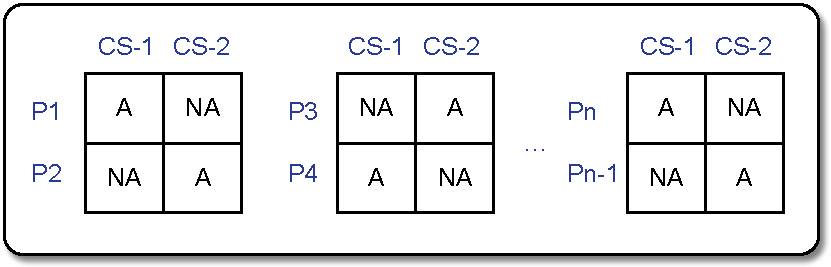
\includegraphics[scale=.50]{images/latin-square.pdf}
      \caption{Latin square design. Each ``square'' corresponds to 
      a replica in our study. Each replica comprises two participants (square rows) 
      and two sets of code snippets (CS-1 and CS-2). We randomly apply the 
      treatments (atom or non-atom code) to the cells of the squares.} 
      \label{fig:latinsquare}
  \end{figure}


Having selected 10 atoms in our first study, we wrote small pieces of code that contained each atom. We also wrote their equivalent snippet without the confusing idioms and constructs, leading to a total of 20 code snippets. In order to reduce the cognitive effort, we decided that each subject would be asked to predict the output of a subset of 10 code snippets, wherein each subset contained five blocks of code that contained atoms of confusion, whilst the remaining five had the atoms removed. The order in which the questions were presented was randomized. By doing this, we were seeking to minimize the chances of subjects being aware that the current listing they were analyzing contained (or not) atoms of confusion.
That is, each respondent of the survey should indicate what would be the outcomes of the code snippets, some of them having atoms of confusion (while other code snippets did not). 
We measured answer correctness and the total time each participant needed to answer the survey's questions.

\subsubsection*{Survey Instrument} 

We implemented our survey as a web application. As part of this 
effort, we carried out an informal pilot whose main objectives were: to spot bugs in the application and in the data collection mechanism; to gain feedback from respondents about the user experience of the application; and to formulate an estimate about how long answering the survey would take on average. Fellow undergraduate students, professional colleagues, and friends took the pilot survey. Some users reported layout defects, and many reported that the landing page did not explain the survey well enough. We also spotted minor issues with our routines to create and populate the Latin Squares. 

We organized the survey in three sections. The first section aims to characterize the subjects, asking for their age, education level, and programming experience. We also included a check button, whose checking meant users agreed that all collected data would be used solely for research purposes. In the second section, we presented to the participants a small set of instructions, where we explained how the survey worked and asked them to dedicate their attention to it. We stressed to participants the importance of not using any aids during the survey, such as online or console interpreters. For each question page, we kept track of whether or not the subjects switched windows. 

The last section of the survey presented a sequence of 10 questions, each containing a code snippet. For each question, there was a text box where the answer should be written. There was also an ``I do not know'' button, which, when clicked, led the subject to the next question. In our setting, ``I do not know'' was treated as a wrong answer. The code snippets were presented as images copied from a text editor, so as to demotivate respondents from resorting to external resources by copying and pasting the code into an interpreter. Upon submitting their answer for a particular question, the subject was automatically led to a similar page, containing another snippet.
    
We decided not to provide feedback about the time students took to answer each question. Nor did we tell them whether their answers were correct or not. Our main concern was to avoid introducing bias for future respondents. Since we posted the survey in a social media platform, if we gave respondents instant feedback, they might post comments on particular atoms, therefore interfering with future participants' thought process.

% \rb{nao acho esse paragrafo necessario} 
% \adriano{o de baixo ne? eu tambem acho}

% As we mentioned before, we first wrote the code listings in a text editor, and took pictures of it. In the case of an atom of confusion that was exclusive to JavaScript, which we called \textit{Automatic Semicolon Insertion} (see Appendix~\ref{sec:appendix-atoms}), it was necessary to remove the syntax highlighter. Even though semicolons at the end of statements are optional to programmers in JavaScript, the interpreter automatically inserts them into the code. Our text editor was incorrectly highlighting a line break after a return statement, even thought it was valid JavaScript syntax. We had thus to turn the highlighter off to take the picture of this atom. 

\subsubsection*{Survey audience}

%% \diego{Esses detalhes são possíveis candidatos para remoção, se precisarmos de espaço}
%% {\color{blue}We invited developers to answer our survey by sending invitations to communities of JavaScript programmers on the Internet. Our initial plan was to try to engage contributors for two major JavaScript projects, namely Node.js and NPM. None of the projects, though, offered a direct way to interact with the community, such as an online discussion forums or mailing list. We would be required to first make contact with the projects' leaders, and only then would we have a chance to approach potential respondents. Due to time constraints, we decided to look for respondents elsewhere.}

We posted the survey on Reddit.\footnote{Reddit is a North American online discussion platform.
Its discussion threads, often called subreddits, are sorted by subject. For our research, we posted information and links to the survey in two JavaScript subreddits.} We explained our research purposes and asked developers of any level of expertise to take the survey. Within twelve hours, we collected more than 150 answers, populating more than 70 replicas of the Latin Squares. We collected significant data on time taken and discrepancies in answer correctness between confusing and non-confusing versions of the snippets. Some inconsistencies arose while building the squares, for instance, when a user quit in the middle of the survey. When this happened, the corresponding row in the square was left incomplete. We considered all squares that contained incomplete rows to be invalid during data analysis and discarded them. Since we had\
 a large enough number of samples, the squares we had to discard did not impact our analysis.

 
\subsection{Interview Study Settings}

To complement our initial survey, we performed semi-structured interviews with professional JavaScript developers, aiming to identify their perceptions regarding code snippets containing atoms of confusion (research question RQ2). We also asked each participant if they knew of any other JavaScript-specific construct that they regarded as being likely to make the code hard to understand (research question RQ3). In this section we detail the protocol we followed to conduct the interviews and to analyze the results.

% Nós realizamos entrevistas semi-estruturas com o objetivo de identificar a percepção dos desenvolvedores com experiência em JavaScript sobre algumas questões relacionadas à compreensão de código em JavaScript. Assim, nesta Seção nós descrevemos os procedimentos adotados para selecionar os participantes para as entrevistas e detalhamos como as entrevistas foram conduzidas. Além disso, detalhamos como os resultados das entrevistas foram analisados.

\subsubsection*{Participants Selection} We invited the participants of the interviews using a snowballing technique. That is, starting from our network of contacts, we invited an initial set of candidates to take part in our survey. From this initial list, we asked for an indication of additional candidates. Our main selection criterion was that all participants should have been working with JavaScript in their daily professional activities. We invited a total of 17 developers, and 15 of them agreed to participate.
%We conducted the interviews for a period of two weeks.


\subsubsection*{Interview Process} We conducted semi-structured interviews using a web conferencing software. We recorded all the interviews with the consent of the participants. On average, the interviews lasted 26.29 minutes, with the shortest one lasting 14.59 minutes and the longest one 43.06 minutes. The main goal of the interviews was to have developers assess whether two versions of code (one with a single atom and another one without the atom) with the same behavior differed concerning program comprehension, and, if so, which version they\
 regarded as the easier one to understand. Two of the researchers conducted the interviews, and a third one listened to all the recordings to cross-validate the collected data.

The interviews had three main parts. In the first one, we asked the developers the following demographic information: name, email, gender, level of education, current job position, JavaScript experience in years and other programming languages they have worked with.
Table \ref{pinterview} summarizes this demographic information.

\begin{table*}[htb!]
\centering
\begin{tabular}
{p{0.4cm}p{0.9cm}p{2.0cm}p{6cm}p{1.9cm} p{4.5cm}}
\toprule
ID & Gender & Level & Role & JS Experience & Other Languages \\ \midrule 
P1 & Male & Graduate & Software Developer & 9 years & Java, PHP, C, Go  
\\ 
P2 & Male & High School & Software Developer & 3 years & Python, Go, Dart, Lua, C++, C\#
\\ 
P3 & Male & Graduate & Software Developer & 4 years & Java, C
\\ 
P4 & Male & Undergraduate & Software Developer & 3 years & Python, C, C++, Java, Go
\\ 
P5 & Male & Master Student & Software Developer & 3 years & Python, SQL
\\ 
P6 & Male & Graduate & Software Architect  & 15  years  & Java, PHP, C, Python , Ruby, C\# and R
\\ 
P7 & Male & Graduate & Software Developer  & 6 years & C, C++, Java, Assembly, Kotlin
\\ 
P8 & Male & PhD & Software Developer & 2 years & Java, Python
\\ 
P9 & Male & Graduate & Business Analyst and Software Developer & 5 years & PHP
\\ 
P10 & Male & Master Student & Business Analyst and Software Developer  & 4 years & Java, C\# and Python
\\ 
P11 & Male & Master Student & Software Architect & 4 years & Java, Erlang, C\#, Cobol
\\ 
P12 & Female & Master & Software Developer  & 1 year & C
\\ 
P13 & Male & Master & Software Developer & 13 years & Java, PHP
\\ 
P14 & Female & Master Student & Software Developer  & 3 years & C, Python, Ruby
\\ 
P15 & Female &  Graduate & Software Developer & 2 years & Java, PHP
\\ \bottomrule
\end{tabular}
    \caption{Demographic information of the participants}
    \label{pinterview}
\end{table*}

In the second part of the interview our aim was to allow the subjects to describe
their JavaScript experience, as well as to allow them to reveal any JavaScript's constructs they regarded as innately confusing. This would allow us to identify potential atom candidates that are more specific to the JavaScript language. Examples of questions we explored in this section include: \emph{Do you think JavaScript is a language that produces code that is hard to understand?} and \emph{Do you regard any particular construct or idiom of the language as
  especially confusing?}


In the third part of the interview, participants were shown the code snippets that were used in the first study. The participants were told both sides of each pair had the same output, and were asked to evaluate which version of the code was easier to understand. The interviewers restrained themselves from introducing bias into the answers by not explaining that one of the sides of each pair contained the atom under investigation. Subjects were just presented the snippets and allowed to take the necessary time to decide on the most readable snippet.

\subsubsection*{Interview Analysis}

We first transcribed each interview and then examined the broad distribution of the answers. Our goal was to build an initial understanding of the participants' perceptions with regards to the challenges to understand JavaScript code in general and JavaScript code with atoms of confusion. We next followed with an open-coding	procedure, highlighting	the main themes and quoting the participant answers, which we show the most important ones in
Section~\ref{sec:interview-results}. Finally, we consolidate the feedback of the participants with respect to the confusion that our set of atom candidates might introduce in JavaScript code.

%\subsection{Third Study: Additional Survey and Interviews}

% \rb{acho que aqui podemos incluir o segundo survey e a segunda
%  rodada das entrevistas, explorando os \'{a}tomos adicionais}


\subsection{Mining JavaScript Software Repositories Settings}

To understand how often atoms of confusion appear in open source projects, and thus answer our fourth research question (\emph{What is the frequency of occurrence of atoms of confusion in practice?}), we mined a set of GitHub open source repositories. To this end, we first collected the most popular GitHub repositories that are primarily written in JavaScript. We measured popularity using the project's stargazers. This metric, available on  GitHub API, represents the number of stars a project received from users of the platform. The same metric has been used in a number of previous studies as a proxy to estimate project's popularity~\cite{gyimesi2019bugsjs,canedo:esem2020}. We then selected the top 100 most popular repositories and removed projects that did not reach the first quartile of the distribution of lines of code.

After filtering out JavaScript project candidates, in the second step we built a curated dataset comprising the top \minedprojects repositories. Examples of projects in this dataset include \textsc{React}, \textsc{Node JS}, and \textsc{AngularJS}. Table~\ref{tab:projects-statistics} presents some statistics about the projects we consider in our research. The size of the projects range from small ones (5543 lines of code) to complex systems with more than 1 MLOC. All projects in our dataset have at least \num{1244} forks and at least \num{23672} stars. We automated all the steps to filter, clone, and collect the statistics from the repositories using Python scripts.

We mined the occurrence of atom candidates from the repositories in our curate dataset using source code queries that we had written using the CodeQL language~\cite{moor:gttse2007}. CodeQL is an object-oriented variant of the Datalog language~\cite{rodriguez2020efficient}, and currently supports researchers and practitioners to query the source code of systems written in different languages (such as \cpplang, Java, and JavaScript). We also automate the process of running the queries and exporting the results to a format that simplifies our
analysis (and also the reproduction of this study). Finally, we carried
out basic descriptive statistics, in order to understand how often the
atoms of confusion appear in practice. 

\begin{table*}[ht]
 \centering
 \begin{tabular}{rrrrrrr}
   \hline
             & Min. & 1st Qu. & Median & Mean & 3rd Qu. & Max. \\ \hline
 Lines of Code           & \num{5543}  & \num{16060.25} & \num{36161.5} & \num{111432.33} & \num{111182.50} & \num{1278405} \\
 Num. of Forks     & \num{1244}   & \num{3029.75} & \num{6078} & \num{8906.24} & \num{9260.50} & \num{68849} \\
 Num. of Contributors  & \num{6}   & \num{184} & \num{285.5} & \num{533.44} & \num{515.75} & \num{4047} \\
 Num. of Stars        & \num{23672} & \num{27055} & \num{34990} & \num{46919.51} & \num{48518} & \num{310935} \\
 
    \hline
 \end{tabular}
 \caption{Some descriptive statistics about the projects used in the MSR study}
 \label{tab:projects-statistics} 
 \end{table*}


